\documentclass[11pt,]{article}
\usepackage{lmodern}
\usepackage{setspace}
\setstretch{1.4}
\usepackage{amssymb,amsmath}
\usepackage{ifxetex,ifluatex}
\usepackage{fixltx2e} % provides \textsubscript
\ifnum 0\ifxetex 1\fi\ifluatex 1\fi=0 % if pdftex
  \usepackage[T1]{fontenc}
  \usepackage[utf8]{inputenc}
\else % if luatex or xelatex
  \ifxetex
    \usepackage{mathspec}
  \else
    \usepackage{fontspec}
  \fi
  \defaultfontfeatures{Ligatures=TeX,Scale=MatchLowercase}
    \setmainfont[]{Arial Nova}
\fi
% use upquote if available, for straight quotes in verbatim environments
\IfFileExists{upquote.sty}{\usepackage{upquote}}{}
% use microtype if available
\IfFileExists{microtype.sty}{%
\usepackage{microtype}
\UseMicrotypeSet[protrusion]{basicmath} % disable protrusion for tt fonts
}{}
\usepackage[margin=15mm]{geometry}
\usepackage{hyperref}
\hypersetup{unicode=true,
            pdfauthor={Xuejiao Zhou and Ben Cole},
            pdfborder={0 0 0},
            breaklinks=true}
\urlstyle{same}  % don't use monospace font for urls
\usepackage{graphicx,grffile}
\makeatletter
\def\maxwidth{\ifdim\Gin@nat@width>\linewidth\linewidth\else\Gin@nat@width\fi}
\def\maxheight{\ifdim\Gin@nat@height>\textheight\textheight\else\Gin@nat@height\fi}
\makeatother
% Scale images if necessary, so that they will not overflow the page
% margins by default, and it is still possible to overwrite the defaults
% using explicit options in \includegraphics[width, height, ...]{}
\setkeys{Gin}{width=\maxwidth,height=\maxheight,keepaspectratio}
\IfFileExists{parskip.sty}{%
\usepackage{parskip}
}{% else
\setlength{\parindent}{0pt}
\setlength{\parskip}{6pt plus 2pt minus 1pt}
}
\setlength{\emergencystretch}{3em}  % prevent overfull lines
\providecommand{\tightlist}{%
  \setlength{\itemsep}{0pt}\setlength{\parskip}{0pt}}
\setcounter{secnumdepth}{5}
% Redefines (sub)paragraphs to behave more like sections
\ifx\paragraph\undefined\else
\let\oldparagraph\paragraph
\renewcommand{\paragraph}[1]{\oldparagraph{#1}\mbox{}}
\fi
\ifx\subparagraph\undefined\else
\let\oldsubparagraph\subparagraph
\renewcommand{\subparagraph}[1]{\oldsubparagraph{#1}\mbox{}}
\fi

%%% Use protect on footnotes to avoid problems with footnotes in titles
\let\rmarkdownfootnote\footnote%
\def\footnote{\protect\rmarkdownfootnote}

%%% Change title format to be more compact
\usepackage{titling}

% Create subtitle command for use in maketitle
\newcommand{\subtitle}[1]{
  \posttitle{
    \begin{center}\large#1\end{center}
    }
}

\setlength{\droptitle}{-2em}

  \title{Future Social Services Institute\\
Visualising the Victorian Care Sector}
    \pretitle{\vspace{\droptitle}\centering\huge}
  \posttitle{\par}
    \author{Xuejiao Zhou and Ben Cole}
    \preauthor{\centering\large\emph}
  \postauthor{\par}
      \predate{\centering\large\emph}
  \postdate{\par}
    \date{s3741909 and s3412349\\
25 / 04 / 2020}

\usepackage{titling}
\usepackage{multirow}
\usepackage{float}
\let\origfigure\figure
\let\endorigfigure\endfigure
\renewenvironment{figure}[1][2] {
    \expandafter\origfigure\expandafter[H]
} {
    \endorigfigure
}
\pretitle{%
  \begin{center}
  \LARGE
  
\includegraphics[width=200mm]{logos.png}\\[\bigskipamount]
}
\posttitle{\end{center}}
\usepackage{booktabs}
\usepackage{longtable}
\usepackage{array}
\usepackage{multirow}
\usepackage[table]{xcolor}
\usepackage{wrapfig}
\usepackage{float}
\usepackage{colortbl}
\usepackage{pdflscape}
\usepackage{tabu}
\usepackage{threeparttable}
\usepackage{threeparttablex}
\usepackage[normalem]{ulem}
\usepackage{makecell}

\begin{document}
\maketitle

{
\setcounter{tocdepth}{2}
\tableofcontents
}
\newpage

\twocolumn

\section{Introduction}\label{introduction}

The Future Social Services Institute (hereon \emph{FSSI}) has been
established cooperatively between the Victorian state government, the
Victorian Council of Social Service (\emph{VCOSS}), and the Royal
Melbourne Institute of Technology (\emph{RMIT}). The objectives of FSSI
are wide-reaching, including (but not limited to) designing educational
programs, assisting in workplace training, researching reforms for the
social services sector, and supporting transformation in not-for-profit
organisations. (Glanz, 2016)

There are numerous industries involved in social services, and these
industries can differ between countries and cultures. As this project
focuses on social services in Victoria and, more broadly, Australia, the
Australian federal government website for the Department of Social
Services includes the following sectors:

\begin{itemize}
\tightlist
\item
  Communities and Vulnerable People
\item
  Disability and Carers
\item
  Families and Children
\item
  Housing Support
\item
  Mental Health
\item
  Seniors
\item
  Women's Safety
\item
  Working Age
\item
  Welfare Reform\\
  (Department of Social Services, 2019)
\end{itemize}

In the Victorian government specifically, social services are bundled
together with health, but include such services as:

\begin{itemize}
\tightlist
\item
  Ageing
\item
  Alcohol and drugs
\item
  Children and families
\item
  Disability
\item
  Housing and homelessness
\item
  Mental health\\
  (Department of Health and Social Services, 2019)
\end{itemize}

More broadly, the Australian Association of Social Workers supports the
definition of social work as laid out by the International Federation of
Social Workers that:

\begin{quote}
\emph{Social work is a practice-based profession and an academic
discipline that promotes social change and development, social cohesion,
and the empowerment and liberation of people. Principles of social
justice, human rights, collective responsibility and respect for
diversities are central to social work. Underpinned by theories of
social work, social sciences, humanities and indigenous knowledge,
social work engages people and structures to address life challenges and
enhance wellbeing.}\\
\quad - International Federation of Social Workers,
\newline \quad \quad ~~July 2014
\end{quote}

Whilst definitions for which industries comprise social services, the
reasons for establishing FSSI and their data needs are much clearer.

\subsection{Background}\label{background}

\subsubsection{An Ageing Population}\label{an-ageing-population}

According to the Australian Institute of Health and Welfare, the number
of Australians aged 65 and over has been increasing steadily since 1927.
In 2017, the total number of Australians over the age of 65 made up 15\%
of Australia's total population, with this proportion only projected to
grow over the coming years. (Australian Institute of Health and Welfare,
2018)\\
Considering Australia's aged population is predicted to increase, it's
reasonable to assume that the number of persons in aged care will
increase as well.

\newpage

\subsubsection{Royal Commission into Aged Care Quality and
Safety}\label{royal-commission-into-aged-care-quality-and-safety}

A myriad of scandals were reported in Australian news services regarding
the care of residents in aged care facilities between 2015 and 2018,
particularly in South Australia. In response to an ABC News Four Corners
investigation in 2018, Prime Minister Scott Morrison announced a Royal
Commission into Aged Care Quality and Safety. (Hutchens, 2018)\\
The terms of reference can be viewed on the Royal Commission's
government website, and cover 7 main objectives for investigation:

\begin{itemize}
\tightlist
\item
  whether aged care is being provided adequately
\item
  specifically, how to provide the best care to younger persons with
  disability in aged care and persons with dementia
\item
  what challenges the aged care sector will face with changing
  demographics and in rural \& regional areas
\item
  what can be done to improve aged care provision
\item
  how to improve the autonomy and independence for patients in care
\item
  sustainability and modernisation of aged care provision\\
  (Royal Commission into Aged Care Quality and Safety, 2018)
\end{itemize}

\subsubsection{NDIS}\label{ndis}

First legislated in 2013, the National Disability Insurance Scheme
(hereon \emph{NDIS}) was established to achieve several objectives, but
primarily to supply funding given to the provision of disability care
(\emph{National Disability Insurance Scheme Act, 2013}). Furthermore,
the NDIS also encompasses regulation and reformation of disabliity care
services in Australia. This funding amounts to AU\$22 billion per year,
which covers half a million Australians with a permanent and significant
disability who are younger than 65 years old. This care isn't solely of
a medical nature, and can also include services that address emotional
health, fitness, education, opportunities to socialise, and more.
(National Disability Insurance Scheme, 2020)

\subsubsection{Disability Royal
Commission}\label{disability-royal-commission}

Similar to the Royal Commission into Aged Care Quality and Safety, a
separate Royal Commission was established in 2019 to investigate
Violence, Abuse, Neglect, and Exploitation of People with Disability
(Prime Minister of Australia, 2019). One of the leading causes for this
Royal Commission was a report that detailed allegations of abuse and
corruption at a Victorian non-profit provider of care for persons with
disability (McKenzie \& Baker, 2014). However, this was just example of
such allegations, with the Royal Commission hearing that persons with
disability in the care of hospitals were vulnerable to misdiagnoses,
medication errors, and generally poor understanding of intellectual
disability (Brown, 2020).\\
As the lengthy name suggests, the terms of reference for the Royal
Commission into Violence, Abuse, Neglect, and Exploitation of People
with Disability have been set deliberately broad so as to encompass a
wide scope of inquiry. As a summary, its objectives are to determine how
care was not provided adequately for persons with disability, and how
the provision of care can be improved. The providers of care is also
broad, including relatives, personal carers, private care facilities,
government care services, hospitals, etc.

\subsubsection{Charitable Organisations}\label{charitable-organisations}

The Australian Charities and Not-for-Profit Commission (\emph{ACNC})
(2019) reported over 57,500 total charities operating or registered
within Australia in the year 2017. Australian charities included in the
ACNC report recorder 1.26 million employees in paid positions, and 3.3
million volunteer roles. Of those more than 57,500 charities, 10.9\% we
found to be operating within the social services sector. Furthermore,
the ACNC reported that 20.5\% of these charities were based in Victoria.
Charities make a sizeable contribution to Australia's workforce and an
equally important contribution to the delivery of social services.

\subsection{Significance}\label{significance}

The social services sector is clearly going to change considerably in
the next few years, which the FSSI cite as one of the primary reasons
for their being established. The FSSI is choosing to focus on 3 pillars
of support to the social services sector; growth, quality, and adaption.
Data collected from a number of sources - ranging from the Australian
Bureau of Statistics to VCOSS to academic studies - will assist FSSI in
assessing how the Victorian social services sector will grow over time,
how the quality of it's services can be maintained and improved, and how
best to both adapt to and inspire the changes that will occur in the
future.

\section{Brief Literature Review}\label{brief-literature-review}

\subsection{Transformation in the Social Services
Sector}\label{transformation-in-the-social-services-sector}

Kyle et al (2018) identified a number of indicators and predictors for
the transformation occurring in the social services sector, as well as
the challenges facing the industry. Chiefly among these were that there
are many women currently working in care roles that are unpaid and
unemployed (United Nations, 2015). Kyle et al (2018) also found that
young and less educated persons faced greater difficulties in finding
employment in paid roles. Further to this, wage growth has not kept up
with rising productivity or salary increases in other sectors,
effectively resulting in pay decreases for the social services sector
(Dew et al, 2016). This is coupled with an ageing workforce that is
exiting the industry, showing real strain on staffing expected for the
social services sector both presently and in the coming years (McKinsey
Global Institute, 2017). Combined with the expected ageing population
stated above, the social services sector needs to embark on rapid change
in order to minimise the strain it will endure in the coming years.

\newpage

\subsection{Data Visualisations in the Social Care
Sector}\label{data-visualisations-in-the-social-care-sector}

In an age of ``\emph{big data}'' , it is essential that digital
transformation be undertaken across social service sectors. Karannasios
(2018) demonstrates that data and analytics can be considered as
important as labour and capital for modern organisations. Community
services sectors should value big data and analytics as currently
maintained by many commercial organisations. Young and Wessnitzer (2016)
state that a good exploratory data analysis begins with the ability to
describe and plot a data set. Thus, visualisations are an effective
method for reviewing the data and can provide valuable insights into
large data sources.

Visualisation techniques are used to present big data in the form of
tables, charts and graphics. It is believed by experts that representing
data visually makes it possible to communicate data effectively and
gives people the opportunity to analyse and examine various datasets
which would otherwise be difficult to understand (Kennedy \& Allen
2017). However, not all visualisation tools are useful in analysing
large datasets or databases. For example, Tableau is a powerful
popularly used visualisation tool but often struggles with complex and
large datasets.

A good visualisation tool is able to explore data interactively with end
users and also assure the interaction quality of users with data
visualisation (Berinato 2016). Tool designers should consider whether
the user is able to adjust properties with the tool's interface, explore
relationships between attributes of their choice and look for links
between different data (Polack 2019). For example, Reinvestment Fund's
Policy Map is a web-based mapping application that allows users to
generate maps at the USA neighbourhood or national level using datasets
on demographics, housing, education etc.

\newpage

\section{Objectives}\label{objectives}

The objective for this project as defined by primary stakeholder FSSI is
to develop a data visualisation tool for exploring ACNC databases, thus
exploring data collected from Australian (specifically Victorian)
charities. Consultation sessions with FSSI futher defined this objective
to comprise two main components: a digital report suitable for hosting
on a website, and an interactive web platform for building bespoke data
visualisations. The desired purpose for both of these solutions is to
facilitate data exploration for FSSI, VCOSS, and industry stakeholders.

\section{Proposed Methodology}\label{proposed-methodology}

\subsection{Digital Report}\label{digital-report}

This project is centred on data that has already been collected and
warehoused by key stakeholders. As such, steps will need to be taken to
verify the data for suitablity, accuracy, and relevance. Once the
appropriate data has been defined via discussion with stakeholders, a
digital report summarising key findings from the latest ACNC dataset
will be compiled. This report will comprise interactive data
visualisations with industry analysis. This will be prepared as a .html
file with R packages \texttt{ggplot2} and \texttt{plotly} used for
visualisations as required. Please see figure 1 for an example of an
interactive \texttt{plotly} chart.

\begin{figure}
\centering
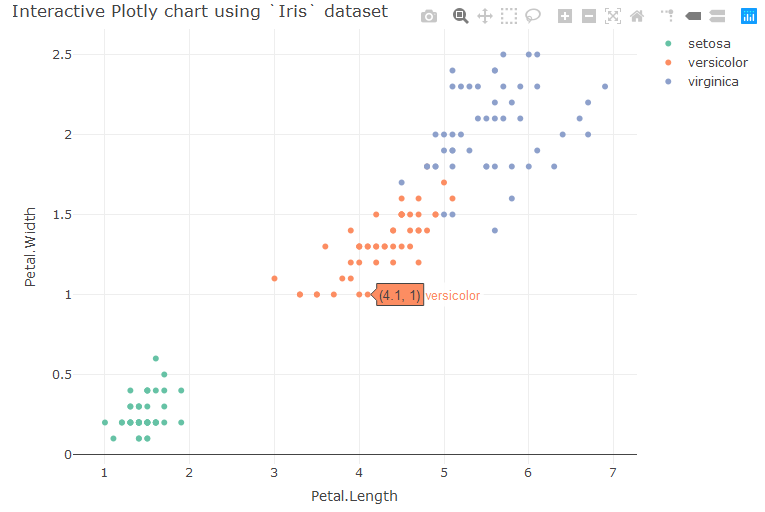
\includegraphics[width=0.48500\textwidth]{Plotly Iris.png}
\caption{A \texttt{Plotly} interactive plot using the Iris dataset}
\end{figure}

\subsection{Visualisation Platform}\label{visualisation-platform}

In addition to this, the ACNC data sets will be used to develop an
interactive Shiny applet that allows users to choose from ACNC data
tables and variables to build their own visualisations. Similar to the
digital report, this solution will also frequently use R packages
\texttt{ggplot2} and \texttt{plotly} for visualisation as well as
\texttt{shiny} or \texttt{dash} for the reactive applet itself.

\section{Project Design}\label{project-design}

This project proposal is the first piece of documentation to be vetted
to FSSI for review. Pending approval from FSSI, the project will
comprise data preparation and cleaning, a digital report, an interactive
visualisation platform, and ultimately a final project report.

\setstretch{1.2}

\subsection{Timeline}\label{timeline}

\begin{table}[H]
\centering\begingroup\fontsize{8}{10}\selectfont
\rowcolors{2}{gray!6}{white}

\begin{tabular}{|>{}l|l|>{}l|}
\hiderowcolors
\hline
\rowcolor[HTML]{caf6f9}  \begingroup\fontsize{8.5}{10.5}\selectfont \textbf{Task}\endgroup & \begingroup\fontsize{8.5}{10.5}\selectfont \textbf{Progress Status}\endgroup & \begingroup\fontsize{8.5}{10.5}\selectfont \textbf{Expected Completion}\endgroup\\
\hline
\showrowcolors
\begingroup\fontsize{8}{10}\selectfont Project Proposal submitted to FSSI\endgroup & \begingroup\fontsize{8}{10}\selectfont Completed\endgroup & \begingroup\fontsize{8}{10}\selectfont 25/04/2020\endgroup\\
\hline
\begingroup\fontsize{8}{10}\selectfont Data Preparation\endgroup & \begingroup\fontsize{8}{10}\selectfont To be commenced\endgroup & \begingroup\fontsize{8}{10}\selectfont 30/04/2020\endgroup\\
\hline
\begingroup\fontsize{8}{10}\selectfont Digital Report\endgroup & \begingroup\fontsize{8}{10}\selectfont To be commenced\endgroup & \begingroup\fontsize{8}{10}\selectfont 24/05/2020\endgroup\\
\hline
\begingroup\fontsize{8}{10}\selectfont Interactive Visualisation Platform\endgroup & \begingroup\fontsize{8}{10}\selectfont To be commenced\endgroup & \begingroup\fontsize{8}{10}\selectfont 06/06/2020\endgroup\\
\hline
\begingroup\fontsize{8}{10}\selectfont Project finalisation and report\endgroup & \begingroup\fontsize{8}{10}\selectfont To be commenced\endgroup & \begingroup\fontsize{8}{10}\selectfont 07/06/2020\endgroup\\
\hline
\end{tabular}
\rowcolors{2}{white}{white}\endgroup{}
\end{table}

\setstretch{1.4}

\subsection{Collaboration Plan}\label{collaboration-plan}

Regular consultation between the project developers and stakeholders
will be required. Prior to the finalisation of this proposal, several
discussions were had between project developers, FSSI, and VCOSS, and
regular meetings will be carried out approximately weekly for the
remainder of the project timeline.

Collaboration within the project development group will be more regular
and less formal, requiring members to regularly communicate when
designing and constructing the above solutions outlined in
\textbf{section 5}.

\subsubsection{Student Contribution
Statement}\label{student-contribution-statement}

Both student members of the project development team have and will
continue to contribute to the project equally.

\newpage

\setstretch{1.25}

\onecolumn

\section{References}\label{references}

\begin{itemize}
\item
  Australian Association of Social Workers, 2020, \emph{What is social
  work?}, AASW - Australian Association of Social Workers, accessed
  11/04/2020,
  \url{https://www.aasw.asn.au/information-for-the-community/what-is-social-work}
\item
  Australian Charities and Not-For-Profit Commission, \emph{Australian
  Charities Report 2017}, accessed 21/04/2020
  \url{https://www.acnc.gov.au/tools/reports/australian-charities-report-2017}
\item
  Australian Institute of Health and Welfare, 2018, \emph{Older
  Australia at a glance}, accessed 12/04/2020,
  \url{https://www.aihw.gov.au/reports/older-people/older-australia-at-a-glance/contents/demographics-of-older-australians/australia-s-changing-age-and-gender-profile}
\item
  Berinato, S, Visualizations That Really Work, Harvard Business Review,
  92--100, June 2016
\item
  Brown, M., 2020, \emph{Intellectually disabled people `unsafe' in
  hospitals, disability royal commission hears}, ABC News, Australia,
  \url{https://www.abc.net.au/news/2020-02-25/hospitals-not-safe-for-intellectually-disabled-inquiry-told/11999170}
\item
  Karanasios, S., 2018, \emph{Chapter Six: Information sharing and
  technological innovation}, Victorian Council of Social Services,
  accessed 18/04/2020,
  \url{http://vcoss.org.au/wp-content/uploads/2018/02/Community-services-of-the-future-FSSI-2018-FINAL.pdf}
\item
  Department of Social Services, 2019, \emph{Our Responsibilities},
  Australian Government, accessed 10/04/2020,
  \url{https://www.dss.gov.au/our-responsibilities}
\item
  Department of Health and Social Services, 2020, *Our Services,
  Victorian Government, accessed 10/04/2020,
  \url{https://www.dhhs.vic.gov.au/our-services}
\item
  Dew, A., Gilroy, J., \& Lincoln, M., 2016, \emph{A Sustainable Rural
  and Remote Workforce for Disability: Research to Action Guide}, Rapid
  Review, Centre for Applied Disability Research
\item
  Fielding, N.G., Lee, R.M. and Blank, G. (2016). The SAGE Handbook of
  Online Research Methods. {[}online{]} Google Books. SAGE. Available
  at:
  \url{https://books.google.com.au/books?hl=en\&lr=\&id=IMWCDQAAQBAJ\&oi=fnd\&pg=PA307\&dq=data+visualisation+\&ots=79d-fEIGUD\&sig=M3xpg9xl0oNSrqa_T9aK6FIWZR4\&redir_esc=y\#v=onepage\&q\&f=false}
  {[}Accessed 17 Apr. 2020{]}.
\item
  Glanz, D., 2016, \emph{RMIT is hosting a new research and teaching
  institute that puts Victoria in the box seat ahead of significant
  change in the delivery of social service.}, Royal Melbourne Institute
  of Technology, accessed 10/04/2020,
  \url{https://www.rmit.edu.au/news/all-news/2016/june/rmit-to-host-social-service-institute}
\item
  Hutchens, G., 2018, \emph{Scott Morrison announces royal commission
  into aged care after string of scandals}, The Guardian Australia,
  accessed 12/04/2020,
  \url{https://www.theguardian.com/australia-news/2018/sep/16/morrison-to-announce-royal-commission-into-aged-care-after-string-of-scandals}
\item
  International Federation of Social Workers, 2014, \emph{GLOBAL
  DEFINITION OF SOCIAL WORK}, accessed 11/04/2020,
  \url{https://www.ifsw.org/what-is-social-work/global-definition-of-social-work/}
\item
  Kyle, L., Macdonald, F., Bentham, E., 2018, \emph{CHAPTER FOUR -
  Workforce of the future for Community Services Industry Plan},
  Victorian Council of Social Services, \textbf{Community services of
  the future, An evidence review}, accessed 19/04/2020,
  \url{http://vcoss.org.au/wp-content/uploads/2018/02/Community-services-of-the-future-FSSI-2018-FINAL.pdf}
\item
  Commonwealth Letters Patent, 2019, Royal Commission into Violence,
  Abuse, Neglect, and Exploitation of People with Disability, accessed
  21/04/2020,
  \url{https://disability.royalcommission.gov.au/publications/commonwealth-letters-patent-4-april-2019}
\item
  McKenzie, N., Baker, R., 2014, \emph{Abusive and corrupt staff
  employed by Yooralla despite warnings, leaked documents and
  whistleblowers claim}, The Age, Victoria Australia, accessed
  21/04/2020
  \url{https://www.theage.com.au/national/abusive-and-corrupt-staff-employed-by-yooralla-despite-warnings-leaked-documents-and-whistleblowers-claim-20141123-11s5wa.html}
\item
  McKinsey Global Institute, 2017, *Briefing note for the Fortune
  Vatican Forum December 2016, McKinsey and Company,
  \url{https://www.scribd.com/document/354361488/MGI-Futureof-Work-Briefing-Note-May-2017}
\item
  National Disability Insurance Scheme, 2020, \emph{What is the NDIS?},
  accessed 12/04/2020,
  \url{https://www.ndis.gov.au/understanding/what-ndis}
\item
  \emph{National Disabliity Insurance Scheme Act 2013},
  \url{https://www.legislation.gov.au/Details/C2013A00020}
\item
  Royal Commission into Aged Care Quality and Safety, 2018, \emph{Terms
  of Reference}, accessed 12/04/2020,
  \url{https://agedcare.royalcommission.gov.au/Pages/Terms-of-reference.aspx}
\item
  Polack, N. (2019). NHS Scotland Open Data: A data visualisation study
  about child health. {[}online{]} Available at:
  \url{http://www.cs.stir.ac.uk/courses/msc/projects/PastProjects/exemplars/Natalie_Polack.pdf}
  {[}Accessed 18 Apr. 2020{]}.
\item
  PolicyMap. (n.d.). PolicyMap. {[}online{]} Available at:
  \url{https://www.policymap.com/} {[}Accessed 18 Apr. 2020{]}.
\item
  Prime Minister, Minister for Families and Social Services, 2019,
  \emph{ESTABLISHMENT OF THE ROYAL COMMISSION INTO VIOLENCE, ABUSE,
  NEGLECT AND EXPLOITATION OF PEOPLE WITH DISABILITY}, accessed
  21/04/2020,
  \url{https://www.pm.gov.au/media/establishment-royal-commission-violence-abuse-neglect-and-exploitation-people-disability}
\item
  United Nations (2015), \emph{World's Women: Trends and Statistics
  2015}, United Nations, New York
\item
  Young, J. and Wessnitzer, J. (2016). Descriptive Statistics, Graphs,
  and Visualisation. Human--Computer Interaction Series, pp.37--56.
\end{itemize}


\end{document}
